\documentclass[../analysisII_notes.tex]{subfiles}
\begin{document}
\section{Aula 06 - 24 de Março, 2025}
\subsection{Motivações}
\begin{itemize}
	\item Calculando integrais;
	\item Propriedades sob Efeito de Operações.
\end{itemize}
\subsection{Calculando integrais}
Na última aula, vimos e provamos o \hyperlink{integral_additivity}{\textit{teorema da aditividade das integrais}}, o qual dizia basicamente que, ao calcular tanto a integral inferior quanto a inferior de uma função num intervalo, podemos pegar qualquer ponto dentro dele e ``recortar a integral'', por meio da soma de integrais, do ponto inicial até o recorte, e dele até o ponto final:
\begin{align*}
	 & \text{(i) } \underline{\intup_{a}^{b}}f = \underline{\intup_{a}^{c}}f + \underline{\intup_{c}^{b}}f \\
	 & \text{(ii) } \overline{\intup_{a}^{b}}f = \overline{\intup_{a}^{c}}f + \overline{\intup_{c}^{b}}f.
\end{align*}
Este processo pode ser repetido quantas vezes quisermos, infinitas vezes. A prova dele seguiu os seguintes passos:
\begin{proof*}
	Provaremos apenas o segundo. Todo o argumento se resume em observar que, para obter a integral superior de f, basta considerar as partições de \([a, b]\) que contêm o ponto c, isto é, aquelas que refinem a partição de três pontos
	\[
		\mathcal{P}_{0}: a < c < b,
	\]
	tal que,
	\[
		\overline{\intup_{a}^{b}}f = \inf_{\mathcal{P}\supseteq \mathcal{P}_{0}}U(f; \mathcal{P})
	\]
	e que, além disso, se \(\mathcal{Q}\) particiona o intervalo \([a, c]\) e \(\mathcal{R}\) o intervalo \([c, b]\), então \(\mathcal{P}=\mathcal{Q}\cup \mathcal{R}\) será uma partição do intervalo \([a, b]\) como um todo, contendo o ponto c.

	Reciprocamente, se \(\mathcal{P}\) particiona \([a, b]\) é uma partição contendo c, então podemos reescrevê-la como
	\[
		\mathcal{P}=(\mathcal{P}\cap [a, c])\cup (\mathcal{P}\cap [c, b]),
	\]
	sendo o primeiro termo em parênteses uma partição de \([a, c]\) e, o segundo, de \([c, b]\); outra forma de ver a mesma coisa dita é que \(\mathcal{P}\) tem a forma
	\[
		\mathcal{P}: \underbrace{a = p_{0} < p_{1} < \dotsc < p_{n}=c}_{\mathcal{Q}} \underbrace{=c< p_{n+1}<p_{n+2}<\dotsc <p_{n+m}=b}_{\mathcal{R}},
	\]
	em que, sim, o c aparece nas duas partições. Com isso,
	\begin{align*}
		U(f; \mathcal{P}) & = \sum\limits_{i=1}^{m+n}M_{i}(p_{i}-p_{i-1})                                              \\
		                  & =\sum\limits_{i=1}^{n}M_{i}(p_{i}-p_{i-1}) + \sum\limits_{i=n+1}^{n+m}M_{i}(p_{i}-p_{i-1}) \\
		                  & = \sum\limits_{i=1}^{n}M_{i}(p_{i}-p_{i-1}) + \sum\limits_{\mathclap{\substack{j=1         \\ ``j=i-n''}}}^{m}M_{n+j}(p_{j}-p_{j-1})\\
		                  & = U(f|_{[a, c]}; \mathcal{Q}) + U(f|_{[c, b]}; \mathcal{R}),
	\end{align*}
	isto é,
	\[
		\Sigma (f|_{[a, c]})+\Sigma (f|_{[c, b]})=\{U(f; \mathcal{P}):\mathcal{P}\supseteq \mathcal{P}_{0}\},
	\]
	e a conclusão segue do lema 2. Portanto,
	\begin{align*}
		\overline{\intup_{a}^{b}}f & = \inf_{}\{U(f; \mathcal{P}):\mathcal{P}\supseteq \mathcal{P}_{0}\}                                                        \\
		                           & = \inf_{}\biggl(\underbrace{\Sigma \bigl(f|_{[a, c]}\bigr)}_{=A} + \underbrace{\Sigma \bigl(f|_{[c, b]}\bigr)}_{=B}\biggr) \\
		                           & = \inf_{}\Sigma \bigl(f|_{[a, c]}\bigr) + \inf_{}\Sigma \bigl(f|_{[c, b]}\bigr)                                            \\
		                           & = \overline{\intup_{a}^{c}}f + \overline{\intup_{c}^{b}}f.\quad \text{\qedsymbol}
	\end{align*}
\end{proof*}
O teorema acima será usado para calcular nossas primeiras integrais de tipos específicos de funções:
\begin{def*}
	Uma função \(f:[a, b]\rightarrow \mathbb{R}\) é a chamada \textbf{função escada} quando existir uma partição
	\[
		\mathcal{P}: a = x_{0} < x_{1} < \dotsc < x_{m}=b
	\]
	do intervalo \([a, b]\) e números reais \(c_{1}, \dotsc , c_{n}\) tais que
	\[
		f(x)=c_{i},\quad x_{i-1}<x<x_{i},\:\forall i=1,2,\dotsc ,n.\quad \square
	\]
\end{def*}
\begin{figure}[H]
	\begin{center}
		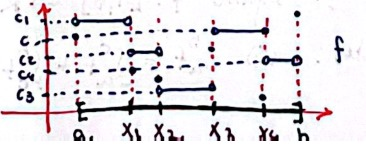
\includegraphics[height=0.5\textheight, width=0.5\textwidth, keepaspectratio]{./Images/step_function_06.png}
	\end{center}
	\caption{função escada representada visualmente.}
	\label{stepfunc06}
\end{figure}
Seguindo a notação da definição, as funções escadas podem assumir \textit{quaisquer} valores nos pontos \(x_{0}, x_1, \dotsc , x_{m}.\)
\begin{example}
	Considere uma função escada com n degraus. Intuitivamente, pela figura e com a ideia da integral como medida de área, esperar-se-á que a área dessa função seja a soma dos retângulos abaixo da integral:
	\[
		\int_{a}^{b}f = \sum\limits_{i=1}^{n}\alpha_{i}(x_{i}-x_{i-1})
	\]
	\begin{figure}[H]
		\begin{center}
			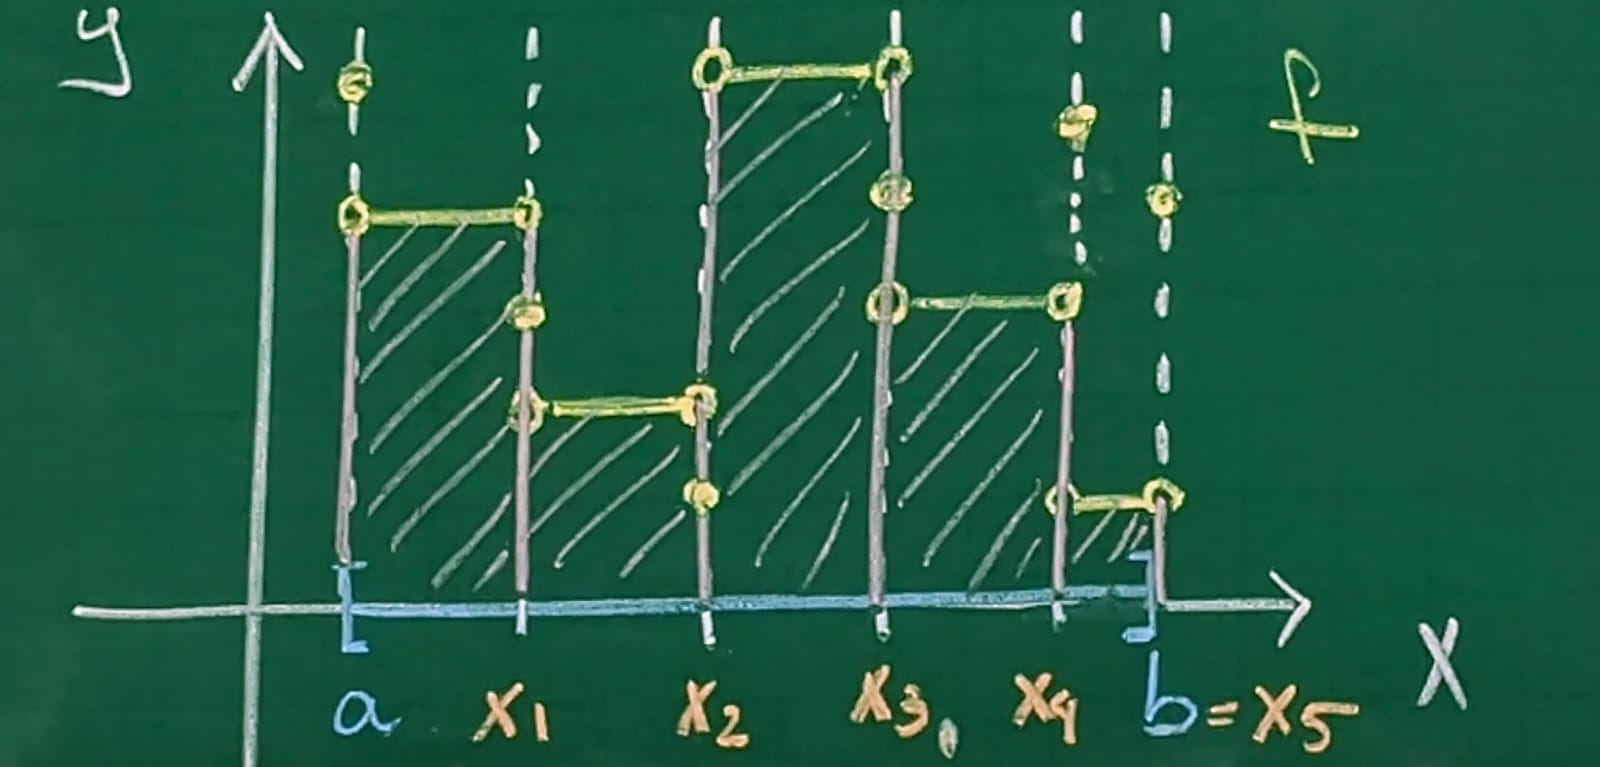
\includegraphics[height=0.5\textheight, width=0.5\textwidth, keepaspectratio]{./Images/step_area_06.png}
		\end{center}
		\caption{a área abaixo de uma função degrau é, intuitivamente, a soma dos retângulos que a compõem.}
		\label{areastep06}
	\end{figure}
	A prova é feita por meio de indução em n, sendo que o caso base \hyperlink{gexample}{\textit{já foi feito antes}}. Tendo o caso base, suponhamos que o resultado vale para o caso n, tal que, definindo \(f_{n}\) como uma função escada com n degraus definida em \([a, b]\), então
	\[
		\int_{a}^{b}f_{n} = \alpha (b-a);
	\]
	provaremos o passo seguinte, ou seja, que a função escada com mais um degrau também satisfaz isto. Para tanto, vamos utilizar o \hyperlink{integral_additivity}{\textit{teorema da aditividade da integral}}, recortando ela no ponto \(x_{n}\):
	\[
		\int_{a}^{b}f_{n+1} = {\color{blue}\int_{a}^{x_{n}}f_{n}} + {\color{red}\int_{x_{n}}^{b} f_{1}},
	\]
	de forma que o termo em azul é o caso suposto, enquanto que o pintado em vermelho nada mais é que uma escada com um degrau, que também já calculamos! Assim,
	\[
		\int_{a}^{b}f_{n+1} = {\color{blue}\sum\limits_{i=1}^{n}\alpha_{i}(x_{i}-x_{i-1})} + {\color{red}\alpha(x_{n+1}-x_{n})},\quad a=x_{0},\: b=x_{n+1}.
	\]
\end{example}
\subsection{Integrais e Operações}
Queremos, agora, abordar as questões referentes à interação entre integrais superiores e inferiores com as operações de soma e multiplicação por escalar - pode-se dizer que queremos estudar a possível linearidade da integral e suas contrapartes. Estreamos este estudo por meio do seguinte lema
\begin{lemma*}
	Se A é um subconjunto limitado da reta real, vale que, para qualquer constante real c, o conjunto
	\[
		cA=\{c \cdot a:\: a\in A\}
	\]
	é limitado. Além disso, valem
	\begin{align*}
		 & \text{(i) }\sup_{}(cA)  = \left\{\begin{array}{ll}
			                                    c \cdot \sup_{}A, & \quad c\geq 0 \\
			                                    c \cdot \inf_{}A, & \quad c < 0   \\
		                                    \end{array}\right.                 \\
		 & \text{(ii) }\inf_{}(cA)  = \left\{\begin{array}{ll}
			                                     c \cdot \inf_{}A,                & \quad c\geq 0 \\
			                                     c \cdot \sup_{}A               , & \quad c < 0   \\
		                                     \end{array}\right.
	\end{align*}
\end{lemma*}
\begin{exr}
	Prove o lema acima.
\end{exr}
Com este lema, enunciamos
\hypertarget{integral_operator}{
	\begin{theorem*}[Operadores com a Integral]
		Sejam \(f, g:[a, b]\rightarrow \mathbb{R}\) duas funções limitadas e considere uma constante real c. Nestas condições,
		\begin{align*}
			 & (I)\: \underline{\intup_{a}^{b}}f + \underline{\intup_{a}^{b}}g \leq \underline{\intup_{a}^{b}}(f+g)\leq \overline{\intup_{a}^{b}}(f+g)\leq \overline{\intup_{a}^{b}}f + \overline{\intup_{a}^{b}}g \\
			\\
			 & (II)\: \overline{\intup_{a}^{b}}(cf) = \left\{\begin{array}{ll}
				                                                 c \overline{\intup_{a}^{b}}f,  & \quad c\geq 0 \\
				                                                 \\
				                                                 c \underline{\intup_{a}^{b}}f, & \quad c<0
			                                                 \end{array}\right. \quad\&\quad \underline{\intup_{a}^{b}}(cf) = \left\{\begin{array}{ll}
				                                                                                                                         c \underline{\intup_{a}^{b}}f, & \quad c\geq 0 \\
				                                                                                                                         \\
				                                                                                                                         c \overline{\intup_{a}^{b}}f,  & \quad c<0
			                                                                                                                         \end{array}\right.                        \\
			\\
			 & (III)\: f(x)\leq g(x),\; \forall x\in[a, b] \Rightarrow \overline{\intup_{a}^{b}}f \leq \overline{\intup_{a}^{b}}g \;\&\; \underline{\intup_{a}^{b}}f \leq \underline{\intup_{a}^{b}}g.
		\end{align*}
	\end{theorem*}}
\begin{proof*}
	(I) Dada uma partição
	\[
		\mathcal{P}: a = t_{0} < t_1 < \dotsc < t_{n} = b,
	\]
	escrevamos
	\begin{align*}
		 & M_{i}(f) = \sup_{}\{f(x):\;x\in x\in[t_{i-1}, t_{i}] \};       \\
		 & M_{i}(g) = \sup_{}\{g(x):\;x\in x\in[t_{i-1}, t_{i}] \};       \\
		 & M_{i}(f+g) = \sup_{}\{(f+g)(x):\;x\in x\in[t_{i-1}, t_{i}] \}.
	\end{align*}
	Pelo corolário do Lema 2 da aula passada,
	\[
		M_{i}(f+g)\leq M_{i}(f)+M_{i}(g) \Rightarrow U(f+g; \mathcal{P})\leq U(f; \mathcal{P}) + U(g; \mathcal{P}).
	\]
	Inicialmente, o esperado era que bastaria passar o ínfimo e obter o resultado, mas isso não funciona! Precisamos considerar \(\mathcal{P},\; \mathcal{Q}\) duas partições quaisquer, tais que
	\[
		\overline{\intup_{a}^{b}}(f+g)\leq U(f+g; \mathcal{P}\cup \mathcal{Q}).
	\]
	Pela desigualdade encontrada, o termo à direita da desigualdade satisfaz
	\[
		U(f+g; \mathcal{P}\cup \mathcal{Q})\leq U(f; \mathcal{P}\cup \mathcal{Q})+U(g; \mathcal{P}\cup \mathcal{Q}),
	\]
	mas, quando refinamos as partições, as somas superiores não crescem! Consequentemente,
	\[
		U(f; \mathcal{P}\cup \mathcal{Q})+U(g; \mathcal{P}\cup \mathcal{Q}) \leq U(f; \mathcal{P})+U(g; \mathcal{Q}).
	\]
	Daí, fixando a partição \(\mathcal{P}\), valerá, para quaisquer outras \(\mathcal{Q}\)'s, a seguinte desigualdade
	\[
		\overline{\intup_{a}^{b}}(f+g) - U(f; \mathcal{P})\leq U(g; \mathcal{Q}).
	\]
	Em outras palavras, o número à esquerda é cota inferior das somas \(U(g; \mathcal{Q})\). Logo,
	\[
		\overline{\intup_{a}^{b}}(f+g)-U(f; \mathcal{P})\leq \overline{\intup_{a}^{b}}g,
	\]
	que podemos reverter para obter
	\[
		\overline{\intup_{a}^{b}}(f+g)-\overline{\intup_{a}^{b}}g \leq U(f; \mathcal{P}).
	\]
	Portanto, agora sim tomando o ínfimo, segue que
	\[
		\overline{\intup_{a}^{b}}(f+g)-\overline{\intup_{a}^{b}}g \leq \overline{\intup_{a}^{b}}f \Longleftrightarrow \overline{\intup_{a}^{b}}(f+g)\leq \overline{\intup_{a}^{b}}f + \overline{\intup_{a}^{b}}g.\quad \text{\qedsymbol}
	\]
\end{proof*}
\end{document}
